\documentclass[12pt, letterpaper]{article}
\usepackage{graphicx} % Required for inserting images
\usepackage{hyperref}
\usepackage{xcolor}
\definecolor{light-gray}{gray}{0.95}
\newcommand{\code}[1]{\colorbox{light-gray}{\texttt{#1}}}
\usepackage{amssymb}
\usepackage{amsmath}
\usepackage[english]{babel}
\usepackage[paper=a4paper,left=20mm,right=20mm,bottom=25mm,top=25mm]{geometry}
\usepackage{wrapfig}
\usepackage{float}
\usepackage{listings}
\title{Sistemi Operativi 1}
\author{Marco Casu}
\date{\vspace{-5ex}}
\begin{document}



\maketitle
\begin{figure}[h]
    \centering{
    
\includegraphics[width=0.7\textwidth ]{images/3OS.png}
    }
\end{figure}
\newpage
\section{Introduzione}
Non esiste una definizione universalmente riconosciuta di sistema operativo, ma una definizione accurata
può essere :
\begin{quote}
    Un sistema operativo, è un implementazione di una macchina virtuale, più facile da programmare rispetto che,
    lavorando direttamente sull'hardware.
\end{quote}
Il sistema operativo (che durante il corso denomineremo come "\textit{OS}"), si interfaccia, o interpone fra
l'hardware ed i programmi ed applicazioni di sistema.
\begin{figure}[h]
    \centering{
    
\includegraphics[width=0.8\textwidth ]{images/osHardwareXApplication.png}
    }
\end{figure}\\
Per progettare un OS bisogna avere delle premesse funzionali per capire cosa includere o no dentro tale
sistema, esistono macchine diverse, con scopi ed esigenze diverse, durante lo svolgimento di tale corso
si tratteranno sistemi operativi per macchine a scopo \textit{generico}. \\Un OS è composto da 2 ingredienti :
\begin{itemize}
    \item \textbf{Kernel} - Il nucleo del sistema, costantemente in esecuzione.
    \item \textbf{Programmi di Sistema} - Tutto ciò che non è il nucleo, ossia i programmi che lo circondano.
\end{itemize}  
Non esiste un sistema operativo adatto a qualsiasi circostanza, è sempre necessario scendere a compromessi (
   concetto di \textbf{trade off}
) per soddisfare i requisiti necessari. In una macchina, un OS svolge diversi ruoli, il primo è quello di
\textbf{arbitro}, ossia, rendere equa ed efficente la gestione delle risorse fisiche a disposizione. Un altro 
ruolo è quello di \textbf{illusionista}, ossia servirsi della \textit{virtualizzazione} per dare la parvenza
all'utente che le risorse a disposizione siano infinite. Un ultimo ruolo è quello di \textbf{collante}, cioè 
interporsi fra software ed hardware per permettergli di comunicare, facendo interagire gli utenti con il
sistema piuttosto che con la macchina direttamente. La componente principale che gestisce un OS è la CPU, 
la memoria ed i dispositivi di Input ed Output (che durante il corso denomineremo come "\textit{I/O}"). Un 
componente da tenere in considerazione è il \textit{bus di sistema}, ossia il mezzo di comunicazione fra 
queste entità, tale bus è suddiviso in :
\begin{itemize}
    \item DATA BUS - trasporta i dati effettivi sulla quale si sta operando.
    \item ADRESS BUS - trasporta l'informazione sull'indirizzo dell'istruzione da eseguire.
    \item CONTROL BUS - trasporta l'informazione sul tipo di operazione da eseguire.
\end{itemize}
I dispositivi di I/O sono composti da i dispositivi fisici in se ed i loro \textbf{device controller}, che ne 
gestiscono la logica interfacciandoli con l'OS tramite i rispettivi \textit{driver}, riservando ad essi dei 
registri per determinarne ed immagazzinarne lo stato e la configurazione, per leggere e scrivere dati da 
essi. Per non fare confusione sul bus quando bisogna comunicare con i dispositivi di I/O, sul bus è previsto
uno switch fisico (M/\#IO) che indica se si vuole comunicare con la memoria o con i device controller. 
A tal proposito, le CPU ha 2 modi per comunicare con questi ultimi : \begin{itemize}
    \item \textbf{port mapped} - I registri dei device controller usano uno spazio di indirizzamento separato
    dalla memoria principale, ma è necessario estendere l'insieme delle istruzioni elementari del linguaggio 
    macchina per per poter comunicare con questo nuovo spazio.
    \item \textbf{memory mapped} - I registri dei device controller vengono mappati sugli stessi indirizzi
    riservati alla memoria principale, tale mappatura avviene all'avvio del sistema, non è quindi necessario
    prevedere nuove istruzioni.
\end{itemize}
\textbf{Direct Memory Access Controller}\\
La CPU controlla \textit{periodicamente} lo stato delle richieste di lettura/scrittura. Un altro modo possibile 
per gestirle è quello delle \textbf{interruzioni}, ossia ogni qual volta che la CPU ha richiesto un operazione
di I/O, quando questa viene completata viene inviato un segnale dal device controller.
Tale segnale, insieme al resto delle comunicazioni fra OS e device controller, avviene su un mezzo di comunicazione
dedicato chiamato \textbf{DMA} (\textit{Direct Memory Access Controller}), ed il suo scopo è quello di occuparsi di trasferire dati dalla memoria ai dispositivi di I/O, 
evitando di delegare tale compito alla CPU, soprattutto quando la quantità dei dati da trasferire è 
considerevole.
\subsection{Job scheduling e Time Sharing}\label{scheduling}
I sistemi operativi moderni devono eseguire contemporaneamente un'ampio numero di programmi ed applicazioni 
(pagine web, editor di testo ecc...). Se in passato i sistemi operativi risiedevano in un ambiente \textbf{uniprogrammato},
ossia che nella memoria era salvato un solo programma che veniva eseguito, adesso gli OS moderni godono di un 
ambiente \textbf{multiprogrammato}, dove vengono mantenuti più processi che vengono caricati in memoria.
Ciascun processo ha determinate istruzioni (jobs) che vengono caricati in memoria, il sistema operativo, come è 
di facile intuizione, è costantemente caricato in memoria.\\
Come organizzare l'esecuzione di più processi? Essi vengono salvati in memoria, se un processo richiede 
dei dati tramite un operazione di I/O, esso viene sospeso finché la richiesta non verrà terminata, nel 
mentre la CPU può "portarsi avanti" il lavoro eseguendo altri processi nel mentre. Usiamo il termine 
\textbf{chiamata bloccante} per indicare una chiamata fatta da un processo che, finchè non è terminata,
impedisce al processo di essere eseguito. Quando si ha un considerevole numero di chiamate bloccanti si rischia
di rallentare troppo l'esecuzione dei programmi, qui agisce lo \textbf{scheduler}, ossia un programma di 
sistema che implementa un algoritmo allo scopo di decidere quale processo deve essere eseguito dalla CPU nel 
momento in cui un altro processo in esecuzione viene arrestato da una chiamata bloccante.
\begin{figure}[h]
    \centering{
    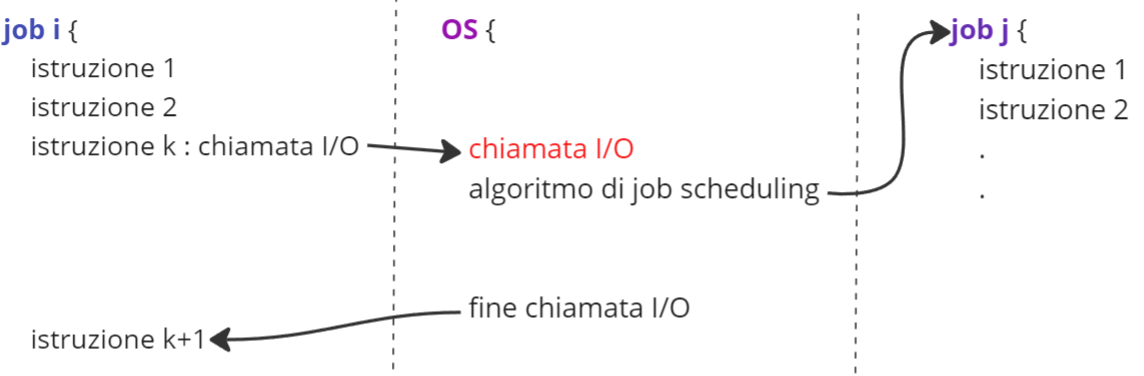
\includegraphics[width=0.7\textwidth ]{images/jobScheduling.png}
    }
\end{figure}
\\Assciurando un buon bilanciamento fra processi in esecuzione e chiamate I/O, tramite il job scheduling
la CPU non si arresterà mai ed avrà sempre un processo in esecuzione. Sorge però un altro problema, nel caso 
dovessimo avere un processo considerevolmente lungo, esso verrà eseguito per un \textit{tempo indeterminato} lasciando 
la CPU sempre occupata, si utilizza quindi un sistema di \textbf{time sharing}, in cui ad ogni processo 
è riservato un \textbf{tempo limitato}, in modo tale che esso se troppo lungo, viene momentaneamente arrestato per 
lasciare spazio ad altri processi (il tempo limite per ogni processo è stabilito dal sistema), essendo tali tempi 
molto bassi per la nostra percezione, tramite il time sharing l'utente avrà un'illusione di \textit{parallelismo} 
(solo apparente dato che una CPU può eseguire un solo processo alla volta).\\
È importante considerare che sospendere un processo per mandarne in esecuzione un altro 
(\textbf{content switch}) ha un suo costo, in quanto bisogna salvare lo \textit{stato} del processo precedente
salvando i valori contenuti nei registri e l'ultima istruzione da eseguire in modo da poterlo poi 
\textit{ripristinare} correttamente, per cui il tempo limitato dal sistema secondo il time sharing non deve 
essere troppo piccolo altrimenti si rischia di fare content switch troppe volte rispetto agli effettivi 
calcoli da eseguire.
\section{Architettura Necessaria per i Servizi dell'OS}\subsection{User e Kernel Mode}
Per mantenere un certo livello di sicurezza, all'interno dell'OS è possibile eseguire istruzioni in due 
modalità differenti, \textbf{user mode} e \textbf{kernel mode}. Alcune istruzioni sono più
\textit{sensibili}, se spostare il contenuto da un registro ad un altro (MOV) può essere fatto senza 
problemi, alcune istruzioni di interruzione dovrebbero richiedere un accesso privilegiato, per questo 
si vuole implementare la \textit{kernel mode}, che ha la possibilità di eseguire qualsiasi istruzione.
Fisicamente, si implementa un \textit{bit} che descrive appunto, tramite i suoi 2 stati, se si sta 
operando da utente, o in modalità kernel. Il sistema, in user mode, non può interagire direttamente 
con l'I/O, e non può manipolare il contenuto della memoria. Se l'utente necessita di eseguire operazioni 
in cui è necessaria la kernel mode, utilizzia le \textbf{system call}, delle chiamate, che permettono 
la momentanea transazione in kernel mode per soddisfare la richiesta, per poi ritornare alla modalità 
utente.
\begin{wrapfigure}{l}{0.25\textwidth}
    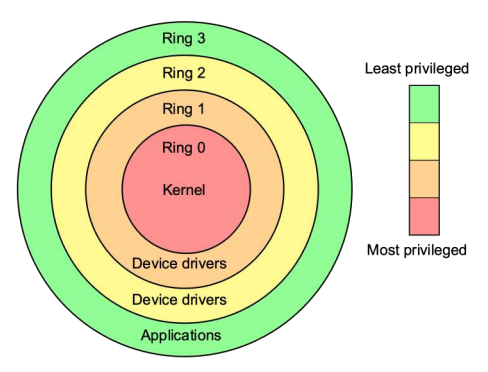
\includegraphics[width=1\linewidth]{images/protectionRings.png} 
    \caption{Protection Rings}
    \label{fig:wrapfig}
    \end{wrapfigure}
     \hphantom{,}\\ \hphantom{,}\\ \hphantom{,}\\Al minimo è necessario un \textit{bit} per i 2 stati, ma è possibile implementarne molteplici 
se si vogliono definire dei \textbf{protection rings}, ossia più stati di privilegi definiti a strati 
dove al livello 0 c'è il kernel, e gradualmente si hanno meno privilegi più il livello è alto. \hphantom{,}\\
\hphantom{,}\\ \hphantom{,}\\ \hphantom{,}\\ \hphantom{,}\\ \hphantom{,}\\
È anche necessario proteggere la memoria, limitanto ogni processo senza dargli la possibilità di poter
operare su tutta la memoria disponibile, a livello hardware si implementano due ulteriori registri, denominati
\textbf{base} e \textbf{limit}, quando un processo è in corso, ad esso verrà riservata una limitata partizione 
di memoria, in \textit{base} sarà contenuto l'indirizzo iniziale dalla quale parte la memoria disponibile, 
ed in \textit{limit} quello finale, in modo da fornire un \textit{range} di memoria utilizzabile. I valori di 
tali registri si aggiornano ad ogni \textit{content switch}, dato che ad ogni processo è assegnato il suo 
range [base,limit].
\subsection{Le System Call}
Come abbiamo già accennato, l'utente non può interagire direttamente con le istruzioni privilegiate, esistono 
appositamente le \textbf{system call} (o chiamate di sistema), esse richiedono al sistema operativo di eseguire 
determinate operazioni (come scrivere dati su un disco o inviare dati ad un interfaccia di rete), quindi esiste una 
lista di operazioni che l'utente può effettuare tramite esse, sono praticamente l'interfaccia tra l'utente ed il 
sistema operativo. Tali richieste sono definite \textbf{trap}, ossia eventi che causano lo switch da 
user a kernel mode, tali \textit{trap} non sono esclusivamente le system call, ma anche le 
\textbf{eccezioni} (errori generati dal software, privilegi assenti per un istruzione o tentata 
divisione per 0), e le \textbf{interruzioni} (errori generati dall'hardware, come la scadenza del tempo 
prefissato per un job tramite il timer).
\begin{figure}[h]
    \centering{
    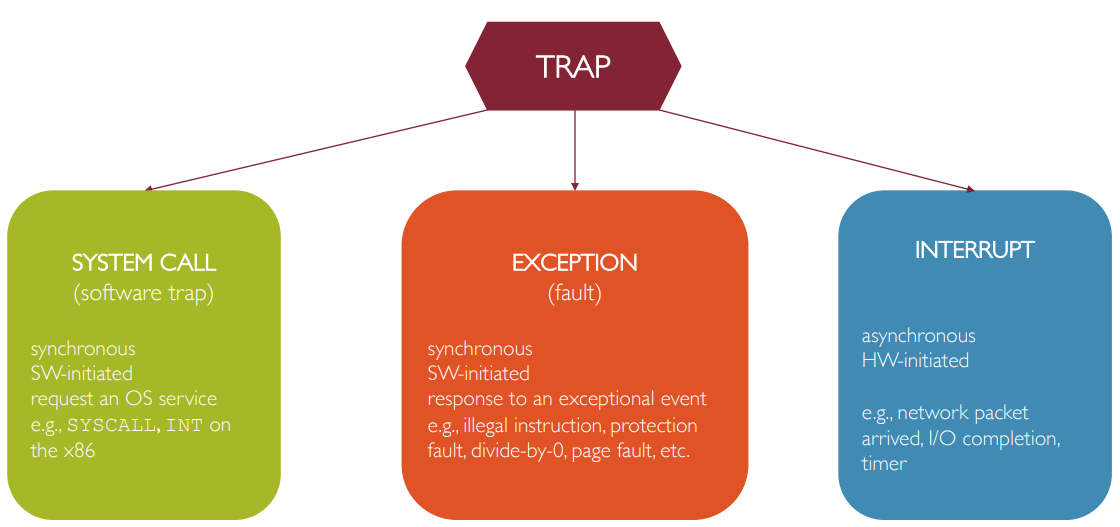
\includegraphics[width=0.7\textwidth ]{images/trapTerminologia.png}
    }
\end{figure}
\\Ci sono 6 categorie principali di system call :
\begin{itemize}
    \item \textbf{Controllo dei processi}
    \item \textbf{Gestione dei file}
    \item \textbf{Controllo dei dispositivi}
    \item \textbf{Manutenzione delle informazioni} 
    \item \textbf{Comunicazione tra processi} - per far comunicare due processi, o si utilizza un canale unico di 
    comunicazione tra i due (\textit{message passing}), oppure si fornisce un area di memoria condivisa tra due processi,
    che andrà poi liberata una volta finita la comunicazione(\textit{shared memory}).
    \item \textbf{Protezione} - forniscono agli utenti accesso temporaneo e limitato ai permessi.
\end{itemize}
\subsection{API per le System Call}
Usando le \textbf{API} (Application Programming Interface) al posto delle system call direttamente, è possibile 
fornite maggiore portatilità, e rendere un programma che necessita delle chiamate di sistema indipendente 
dall'hardware. Un API fornisce una libreria per un linguaggio di programmazione di alto livello (come il \textit{C}), 
che ci permette di chiamare funzioni che eseguiranno delle chiamate di sistema.
\begin{figure}[h]
    \centering{
    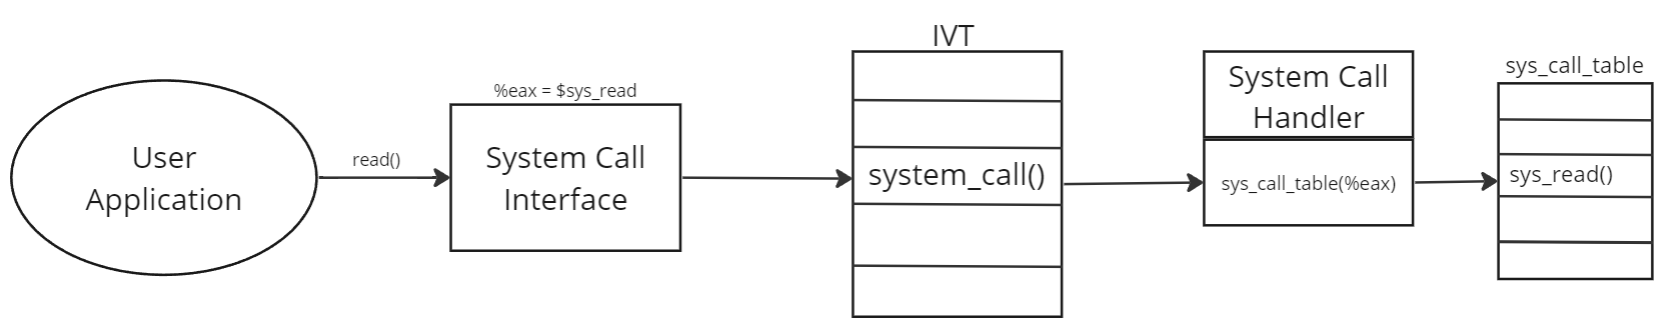
\includegraphics[width=0.9\textwidth ]{images/syscallFlow.png}
    }
\end{figure}
\newpage
Quando un utente chiama una funzione che richiede una syscall, viene generata un'interruzione, poi in un registro apposito 
(nell'immagine sovrastante "\textit{\%eax}") viene salvato il codice di quella specifica chiamata,
il segnale viene poi mandato alla \textbf{IVT} (Interrupt Vector Table), ossia un vettore all'interno 
del kernel che assegna ad ogni interruzione una casua. Quindi l'IVT, capisce che si tratta di una system call 
e manda il segnale al \textit{System Call Handler}, che si occupa di leggere il contenuto del registro 
prima citato ("\textit{\%eax}"), ed in base al codice, richiamare dalla \textit{System Call Table} la chiamata 
corretta.\\\hphantom{.}\\
Spesso, i parametri da passare non si limitano al codice identificativo della system call. Esistono 3 
diversi modi di passare parametri al sistema operativo :
\begin{itemize}
    \item Salvare parametri in dei \textbf{registri} (ma potrebbero esistere più parametri che registri).
    \item Salvare i parametri in \textbf{blocchi} o "tavole" in un'area di memoria dedicata, passando come 
    parametro nei registri l'indirizzo di tali blocchi.
    \item Passare i parametri inserendoli (\textit{push}) in uno \textbf{stack} dal programma, per poi farli 
    riprendere dallo stack (\textit{pop}) direttamente dal sistema operativo.
\end{itemize}
Il metodo migliore risulta quello dei \textit{blocchi} o dello \textit{stack}, dato che non hanno limiti sulla 
quantità di parametri che si possono possibilmente passare.\\\hphantom{.}\\
Le chiamate di I/O eseguite dalle system call possono essere \textbf{bloccanti} o \textbf{non bloccanti},
le chiamate bloccanti, interrompono il flusso del processo, lasciandolo in "stallo" finchè non si
riceveranno i dati richiesti dalla chiamata. Le chiamate non bloccanti invece, richiedono dati tramite 
le chiamate senza però interrompere il processo, sono quindi più difficili da implementare in quanto 
il programmatore deve considerare che dopo la chiamata, i dati richiesti potrebbero non essere 
da subito disponibili.\\\hphantom{.}\\
Come si è accennato precedentemente, risulta utile a livello fisico implementare un \textbf{timer} che 
segna semplicemente l'orario del giorno corrente (detto \textit{time stamp}), esso è utile allo 
\textit{scheduler}\ref{scheduling}, ad esempio, può generare un interruzione ogni 100 \textit{microsecondi}, in modo che 
lo scheduler possa prendere il sopravvento sul processo per poi decidere quale altro job va eseguito.\\\hphantom{.}\\
Alcune istruzioni sono dette \textbf{atomiche}, ossia, non possono essere fermate dalle interruzioni, le architetture 
che implementano tali sitruzioni devono far si che esse vengano eseguite per intero, piuttosto, vengono
totalmente abortite. Per eseguirle è possibile definirle nel linguaggio macchina come istruzioni speciali 
che sono nativamente eseguite in maniera atomica, oppure, è possibile \textit{disabilitare} momentaneamente 
tutte le interruzioni.
\subsection{La Memoria Virtuale}
La \textbf{memoria virtuale} è un \textit{astrazione} della memoria fisica, da l'illusione ad un processo di 
avere illimitato spazio di memoria per lavorare, e consente ad esso di non essere totalmente caricato 
in memoria, caricandolo appunto nella memoria virtuale. Tale memoria è implementata sia a livello 
hardware(MMU) che software(OS) :
\begin{itemize}
    \item \textbf{MMU} - è il componente che si occupa di tradurre gli indirizzi virtuali in indirizzi fisici.
    \item \textbf{OS} - è responsabile di gestire lo spazio degli indirizzi virtuali.
\end{itemize}
Un sistema a 64 \textit{bit}, è capace di indirzzare \(2^{64}\) \textit{bytes}, gli indirizzi virtuali sono 
suddivisi in blocchi della stessa dimensione, chiamati \textbf{pagine}, le pagine che non vengono caricate 
nella memoria principale, vengono salvate sul disco. Facendo ciò si fornisce ad un processo una quantità \(n\) di 
indirizzi virtuali, che sono salvati sia in memoria che su disco, essi vengono mappati tramite quella che si chiama 
\textbf{page table}, e si utilizza anche una cache chiamata \textbf{TLB} (Translation Look-aside Buffer), che salva 
i recenti "indirizzamenti" per potervi accedere più rapidamente. L'OS deve considerare quali pagine sono 
salvate sul disco, e quali sulla memoria principale.
\section{Design ed Implementazione di un Sistema Operativo}
La struttura interna di un sistema operativo può variare largamente in base alle necessità di utilizzo 
di tale sistema, è necessario separare quelle che sono le \textbf{politiche} del sistema 
(Le funzioni che deve svolgere) dal suo \textbf{meccanismo} (La possibile implementazione di tali funzioni).
Tale distinzione ci permette di rendere l'OS più flessibile alle modifiche, riusabile per implementare nuove 
politiche, e stabile. I primi sistemi operativi erano totalemnte implementati in linguaggio macchina, ciò 
consentiva ad essi di essere molto efficenti, di contro però, erano limitati esclusivamente all'hardware sulla 
quale erano scritti. I sistemi operativi odierni hanno esclusivamente una piccola porzione scritta in 
linguaggio macchina, il corpo principale è scritto in \textit{C}, ed i programmi di sistema possono essere scritti 
in \textit{C++}, ed altri linguaggi di scripting come \textit{Python}. Un OS dovrebbe essere partizionato 
in sotto-sistemi, ognungo con compiti ben definiti. Esistono varie strutture di sistema operativo :
\begin{itemize}
    \item \textbf{Simple Structured} - Un sistema non modulare, nella quale non esiste distinzione tra 
    user e kernel. Risulta facile da implementare, ma pecca di rigidità e sicurezza. Un esempio di un OS che 
    adopera tale struttura è \textit{MS-DOS}.
    \item \textbf{Kernel Monolitico} - Un sistema strutturato in modo che sia tutto un grande ed unico processo, con
    tutti i servizi che vivono nello stesso spazio di indirizzamento. Risulta efficente,
    ma essendo un unico processo non ci sono limiti di visibilità tra diverse componenti, risulta 
    quindi poco sicuro. Un esempio di un OS che adopera tale struttura è \textit{UNIX}.
    \item \textbf{Layered Structured} - Un sistema diviso in \(n\) strati, dove il livello 0 rappresenta l'hardware, 
    ed ogni livello \(k\) implenta delle funzionalità che potranno essere riutilizzate dal livello \(k+1\) per 
    implementare nuovi programmi. Essendo modulare, risulta portatile, ma bisogna implementare dei canali di 
    comunicazione fra i vari strati.
    \item \textbf{Micro Kernel} - È l'opposto del \textit{Kernel Monolitico}. Nel kernel si inseriscono 
    esclusivamente le funzionalità di base, tutto il resto sarà gestito dalle applicazioni a livello utente. Risulta
    sicuro ed estendibile, ma pecca nella comunicazione. 
    \item \textbf{Loadable Kernel} - Ogni componente è separata, l'approccio risulta simile ai linguaggi 
    di programmazione \textit{object-oriented}. I moduli vengono caricati separatamente all'interno del 
    kernel. Ogni componente comunica con le altre tramite un interfaccia, è simile al \textit{Layered Structured},
    ma più flessibile.
\end{itemize}
È importante in base alla struttura utilizzati, provvedere al giusto hardware da implementare. I sistemi 
moderni utilizzano per lo più approcci ibridi.\newpage
\section{La Gestione dei Processi}
Definiamo la differenza tra \textbf{programma} e \textbf{processo} :
\begin{itemize}
    \item Programma - rappresenta l'eseguibile di un certo applicativo, contiene le istruzioni da eseguire ed 
     è contenuto sul disco fisso. 
     \item Processo - rappresenta l'istanza del programma che viene avviato e caricato sulla memoria principale,
     una volta avviato, l'OS si occuperà di tale processo. 
\end{itemize}
Quindi un programma viene \textit{istanziato} in un processo, che è un entità dinamica e viene eseguito 
dalla CPU, ogni processo è un entità indipendente, e possono coesistere due processi istanza dello stesso
programma. Ad ogni processo viene assegnata la sua quantità di memoria disponibile, e le sue istruzioni sono 
eseguite in maniere sequenziale. Il sistema operativo si occupa di creare, distruggere, e gestire gli stati 
dei processi, dedica ad essi la stessa quantità di memoria virtuale, ed il numero di indirizzi disponibili dipendono 
dall'architettura della macchina (ad esempio, con un processore a 32 \text{bit}, si hanno \(2^32\) indirizzi disponibili).
\\\hphantom{.}\\
Quando si crea un processo, ad esso viene assegnata una quantità di memoria divisa in 5 unità logiche :
\begin{itemize}
    \item \code{Text} - contiene le istruzioni eseguibili, ossia il risultato della compilazione.
    \item \code{Data} - contiene le variabili globali o statiche inizializzate.
    \item \code{Data} - contiene le variabili globali o statiche non inizializzate, o inizializzate a 0.
    \item \code{Stack} - struttura LIFO utilizzata per memorizzare i dati ed i parametri necessari alle chiamate di funzioni.
    \item \code{Heap} - struttura dati utilizzata per l'allocazione dinamica della memoria.
\end{itemize}
Per ogni processo quindi, esiste tale area di memoria suddivisa in 5 unità. Lo \textbf{Stack} ha su di esso due 
operazioni, \code{push()} e \code{pop()}, ed un registro dedicato chiamato \textit{Stack Pointer} memorizza 
l'indirizzo alla cima dello stack. Ogni funzione utilizza una porzione dello stack che viene denominata 
\textbf{Stack Frame}, quindi quando si chiamano funzioni dentro altre funzioni, coesisteranno simultaneamente 
più stack frame, anche se esclusivamente uno di essi sarà attivo, ossia quello sulla quale risiede lo 
stack pointer (lo stack "cresce" verso il basso, quindi l'ultima funzione chiamata sarà quella attiva). 
\\\hphantom{.}\\ Lo stack frame contiene :\begin{itemize}
    \item Parametri della funzione ed indirizzo di ritorno
    \item Puntatore al precedente dello stack frame precedente
    \item Variabili locali
\end{itemize}
Quando si chiama una funzione che richiede dei parametri,
essi verrano inseriti (\code{push()}) nello stack, il valore dello stack pointer verrà aggiornato, e verrà inserito nello 
stack anche l'indirizzo dell'istruzione di ritorno. Il problema è che lo stack pointer viene aggiornato ogni 
volta che si chiama una nuova funzione, quindi si usa un altro puntatore detto \textit{Base Pointer} sul fondo 
dello stack, che rimane fisso per ogni stack frame senza aggiornarsi, differentemente dallo stack pointer che per 
forza di cosa, si aggiorna ogni qual volta viene aggiunto un nuovo valore.\newpage \subsection{Stati di un Processo}
Un processo in esecuzione può ritrovarsi in uno dei seguenti 5 \textbf{stati} : \begin{itemize}
    \item \code{new} - Il sistema operativo ha indirizzato le strutture per eseguirlo.
    \item \code{ready} - Il processo ha tutte le risorse necessarie per iniziare o ricominciare ad essere eseguito.
    \item \code{running} - Il processo è in esecuzione sulla CPU.
    \item \code{waiting} - Il processo è sospeso, in attesa che venga soddisfatta una chiamata/richiesta che necessita per poter continuare.
    \item \code{terminated} - Il processo è concluso, l'OS può liberare la memoria dalle risorse che utilizzava.
\end{itemize}
\begin{figure}[h]
    \centering{
    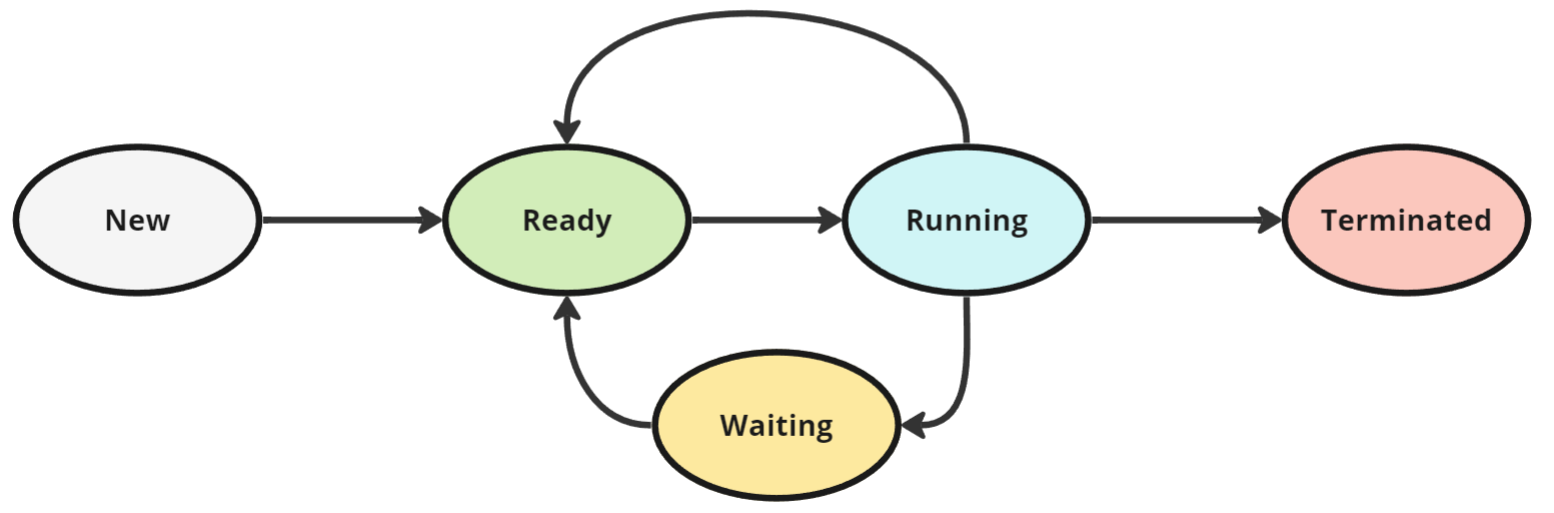
\includegraphics[width=0.7\textwidth ]{images/processStates.png}
    }
\end{figure}
\subsection{Creazione dei Processi}
Il sistema operativo per creare nuovi processi utilizza delle opportune chiamate di sistema. Per convenzione, 
un processo \textit{Parent} (detto anche padre) è quello dalla quale si esegue la chiamata per generare nuovi processi, detti 
\textit{Figli}. Ogni processo ha d.ue valori interi utilizzati per identificare se stesso: \code{PID}, ed 
il suo parent : \code{PPID}. In sistemi come Unix, il process scheduler ha come PID=0, esso inizializza 
come prima cosa un processo noto come \code{init}, che ha PID=1, e si occuperà di creare tutti i processi, sarà 
quindi il parent primario. I processi vengono creati tramite una chiamata di sistema denominata \code{fork()}.
Ogni processo crea più figli, generando una struttura gerarchica ad albero.\\
\hphantom{}\\ La chiamata \code{fork()} nello 
specifico, non crea un nuovo processo, ma crea un processo \textit{clone}, identico a quello chiamante, si utilizza 
poi una chiamata \code{exec()}, che prendendo come parametri l'indirizzo in memoria di un determinato programma, 
sostituirà al processo corrente le istruzioni del programma nuovo che si vuole eseguire. Sarà quindi la congiunzione 
di tali chiamate \code{fork()} ed \code{exec()} a generare un nuovo processo.
\\\hphantom{}\\ 
Quando un processo padre genera un figlio, ha due possibili opzioni :\begin{itemize}
    \item Arrestare la sua esecuzione, ed attendere che il processo figlio appena generato termini prima di ricominciare,
    tramite la chiamata \code{wait()}.
    \item Continuare la sua esecuzione, in maniera concorrente con il suo processo figlio.
\end{itemize}
Vediamo come un programma si occupa di generare un nuovo processo tramite la chiamata di sistema :\newpage
\begin{lstlisting}[language=C]
    #include <sys/types.h>
    #include <stdio.h>
    #include <unistd.h>
    
    int main(){
        pid_t pid;
        /* fork a child process */
        pid = fork();

        if(pid<0){
            /* error occurred */
            fprint("Fork Failed");
            exit(-1);
        }

        else if(pid==0){
            /* child process */
            execlp("bin/ls","ls",NULL);
        }

        else{
            /* parent process */
            wait(NULL);
            printf("Child Complete");
            exit(0);
        }
    }
\end{lstlisting}
Si osservi il codice sopra mostrato. Quando viene eseguito un \code{fork()} e creato un clone, i due processi 
padre e figlio differiranno esclusivamente per il loro PID. La funzione \code{fork()} ritorna il PID del 
processo appena clonato(quindi il padre avrà salvato nella variabile, il PID del figlio)
, il processo figlio, avrà la variabile pid=0, per questo si entrà nel blocco 
di codice che si occuperà di fare l'\code{exec()} sostituendo le istruzioni con quelle del 
programma presente all'indirizzo \code{"bin/ls"}, generando così un nuovo processo. Se il PID è diverso da 0, 
il programma eseguirà una \code{wait()}, aspettando che il processo figlio termini, prima di ricominciare.
\begin{figure}[h]
    \centering{
    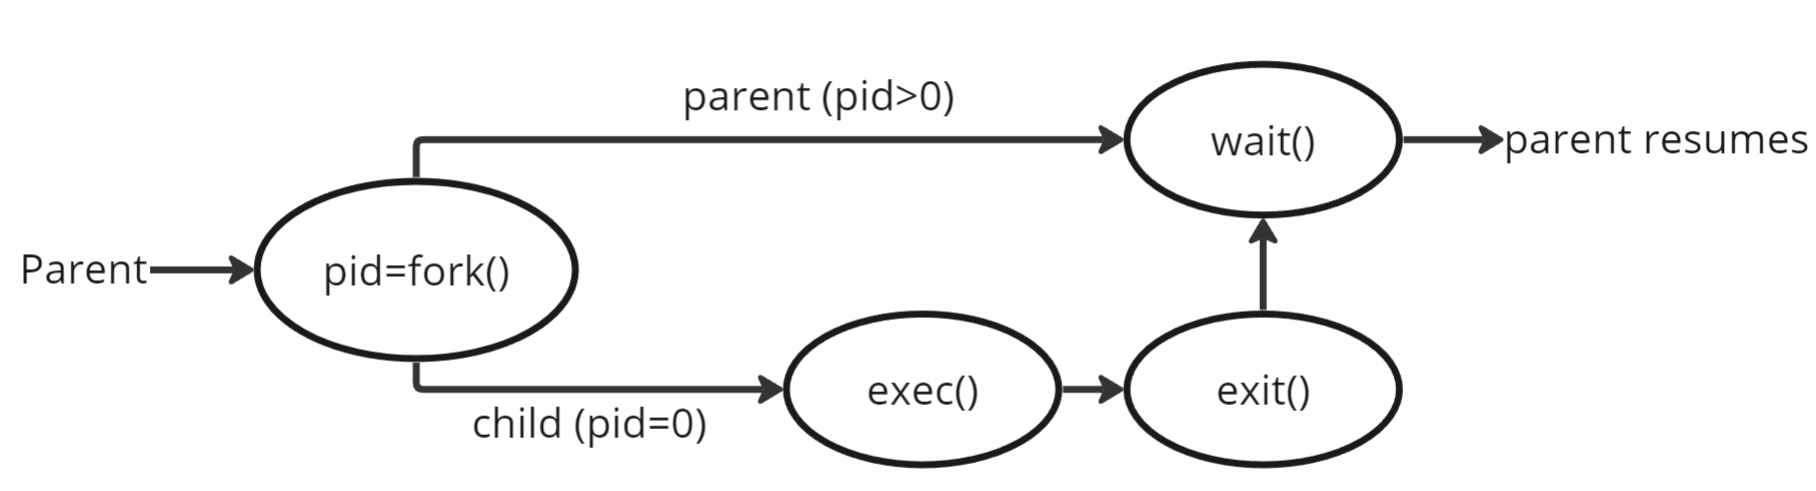
\includegraphics[width=0.9\textwidth ]{images/forkGraph.png}
    }
\end{figure}
Sarà quindi il programma scritto dall'utente a dover implementare la logica adeguata (tramite la 
lettura dei PID) per capire se il processo attualmente in esecuzione è quello padre o quello figlio.
\\\hphantom{}\\ 
Un processo può esplicitamente richiedere la sua terminazione tramite la chiamata di 
sistema \code{exit()}, dando un codice di uscita, che per convenzione è 0 quando tale processo 
ha terminato la sua esecuzione senza errori, altrimenti -1, oppure può essere terminato in maniere 
forzata dal suo processo padre. Un processo non può esistere senza padre,
se un processo padre termina ma vi sono ancora dei processi figli in esecuzione, essi, detti 
processi \textit{orfani}, vengono ereditati dal processo \code{init}, che si occuperà di terminarli.
Quando un processo termina, lo spazio dedicato alle sue risorse viene liberato.
\subsection{Scheduling dei Processi}
Un sistema operativo deve far conto a due obbiettivi : \begin{itemize}
    \item far si che la CPU stia costantemente eseguendo processi 
    \item avere un t empo di risposta accettabile per i programmi che interagiscono con l'utente
\end{itemize}
Lo scheduler si occupa di decidere quale processo eseguire venendo in contro a tali obbiettivi, anche se 
essi possono entrare in conflitto fra loro. Il sistema operativo salva tutti i PCBs\footnote{
 Process Control Block
} dei processi in delle code, ci sono 5 code, una per ogni possibile stato. Quando un processo cambia stato, 
il suo PCB viene eliminato dalla coda precedente ed inserito nella nuova coda corrispondente. Ovviamente, 
nella \textit{Running Queue} vi può essere un solo processo per volta (in sistemi con architetture single core).
Nelle altre code, non ci sono limiti teorici di dimensioni.
\\\hphantom{}\\ 
Esistono due tipi di scheduler.\begin{itemize}
    \item Il \textbf{long-term scheduler} si occupa di selezionare i processi da eseguire dalla memoria secondaria 
    (ad esempio, il disco) e di caricarli in memoria principale, viene eseguito poco frequentemente.
    \item Lo \textbf{short-term scheduler} nvece, si occupa di selezionare i
     processi dalla coda dei pronti e di assegnarli alla CPU per l'esecuzione, viene eseguito molto frequentemente,
     circa ogni 50-100 millisecondi.
\end{itemize}
Abbiamo già definit l'operazione di \textit{Content Switch}, ossia quella di interrompere un processo per 
eseguirne un altro. Tale operazione risulta costosa in termini computazionali, dato che è necessario salvare 
lostato del processo da interrompere e caricare lo stato del processo da eseguire dai loro rispettivi 
PCB. Il content switch è quindi operazione da eseguire solo quando necessario, quando avviene un interruzione, oppure 
quando un processo impiega troppo tempo generando un interruzione del timer. I processi che utilizzano principalmente 
la CPU per eseguire esclusivamente calcoli (talvolta pesanti), che quindi richiedono più tempo per essere 
completati, senza però fare richieste di I/O, sono detti \textit{CPU-bound processes}.
\\\hphantom{}\\ 
Il tempo che impiega la CPU per fare content switch è "sprecato" dato che non si stanno effettuando 
calcoli utili all'esecuzione dei processi, quindi a seconda delle disponibilità, è possibile implementare 
un quanto di tempo massimo dedicato ad ogni processo, a seconda delle esigenze :\begin{itemize}
    \item Un quanto di tempo minore farà si che si eseguiranno più content switch, aumentando la responsività.
    \item Un quanto di tempo maggiore risulterà in meno content switch, minimizzando il tempo perso della CPU, massimizzandone
    il suo utilizzo.
\subsection{Comunicazione fra processi}
\end{itemize}


















\end{document}
\color{red} \textbf{Continuare da }: Slide :05-Basics-of-OS-Process-Management.pdf pagina 71